\documentclass{article}
\usepackage{graphicx}
\graphicspath{{./}{../FIGs/}{../Logos/}}
\ifx\HCode\Undef
\DeclareGraphicsExtensions{.pdf,.png}
\else
\usepackage{tex4ht}
\DeclareGraphicsExtensions{.svg, .png, .jpg}
\fi
\usepackage{hyperref}
\usepackage{color}

%\renewcommand{\rmdefault}{ptm}
%\renewcommand\familydefault{\sfdefault}

\newcommand{\luxunda}{%
\begin{tabular}{c}
  Crist\'obal Medina L\'opez, \\
  Juan Pablo Garc\'ia Ortiz and \\
  Juan Alvaro Mu\~noz Naranjo. \\
  ~\\
  \href{http://www.luxunda.es/}{Luxunda SA}
\end{tabular}
}

\newcommand{\SAL}{%
\begin{tabular}{c}
  Leocadio Gonz\'alez Casado and \\
  Vicente Gonz\'alez Ruiz.\\
  ~\\
  \href{http://www.hpca.ual.es/}{SAL, UAL}
\end{tabular}
}

\author{%
Crist\'obal Medina L\'opez, Juan Pablo Garc\'ia Ortiz and Juan Alvaro Mu\~noz Naranjo,\\\href{http://www.luxunda.es/}{Luxunda SL}. \\
~\\
Leocadio Gonz\'alez Casado and Vicente Gonz\'alez Ruiz,\\\href{http://www.hpca.ual.es/}{SAL, UAL}.
}

%\begin{tabular}{cc}%
%  \luxunda &  \SAL %
%\end{tabular}%

\newcommand{\thankss}{
%{{{

  \vbox{
    \ifx \HCode\Undfef
    \else
    \HCode{<div style="text-align:center;">
      <img width=800 src="FIGs/thanks.svg" align="top"/>
      </div>
    }
    \fi
  }

%}}}
}

\title{IP-TV over P2PSP Teams}
\date{Nov 18, 2014 \\~\\ \url{http://slides.p2psp.org/2014-11-Jornada-Contenidos-Digitales-UAL} \\~\\ \thankss}

\begin{document}
% Family       Font Name
% pag          Avant Garde *
% fvs          Bitstream Vera Sans
% pbk          Bookman
% bch          Charter
% ccr          Computer Concrete
% cmr          Computer Modern
% pcr          Courier
% mdugm        Garamond
% phv          Helvetica *
% fi4          Inconsolata
% lmr          Latin Modern
% LinuxBiolinumT-OsF     Linux Biolinum (formerly 'fxb' in older package versions)
% LinuxLibertineT-OsF    Linux Libertine (formerly 'fxl' in older package versions)
% pnc          New Century Schoolbook
% ppl          Palatino
% ptm          Times
% uncl         Uncial
% put          Utopia
% pzc          Zapf Chancery

%\fontfamily{pag}\selectfont
\fontfamily{phv}\selectfont
%\sffamily
%\def\normalfont{\sffamily}
%\renewcommand{\familydefault}{cmss} \
%\renewcommand{\familydefault}{\sfdefault}
%\selectfont

\maketitle

%\section*{Slide's URL}
%\begin{center}
%  \href{http://www.p2psp.org/slides/}{http://www.p2psp.org/slides/Jornada-CPC-UAL-2014}
%\end{center}

%\begin{center}
%  
\includegraphics[width=2cm]{../Logos/thanks.png}
%\end{center}

% \ifx \HCode\Undfef
% \else
%   \HCode{<HR width=100\% align="left">}
% \fi
\clearpage
\newpage
\tableofcontents

\section{Digital Video Broadcasting (DVB)}
% \ifx \HCode\Undfef
% \else
%   \HCode{<div class="vbox"></div>
% <div class="hbox">}
% \fi

\ifx \HCode\Undfef
%\begin{center}
%  \includegraphics[width=1.0\textwidth]{DVB}
%\end{center}
\else
\HCode{
  <div style="text-align:center;">
    <img height="700" src="FIGs/DVB.svg" />
  </div>
}
\fi

% \ifx \HCode\Undfef
% \else
%   \HCode{</div>}
% \fi

\section{Internet Protocol (IP)}
\ifx \HCode\Undfef
%\begin{center}
%  \includegraphics[width=1.0\textwidth]{world-internet}
%\end{center}
\else
\HCode{
  <div style="text-align:center;">
    <img height="500" src="FIGs/world-internet.svg" />
  </div>
}
\fi

\section{Video on Demand over the Internet (IP-VoD)}
\ifx \HCode\Undfef
%\begin{center}
%  \includegraphics[width=1.0\textwidth]{spain-IPVoD}
%\end{center}
\else
\HCode{
  <div style="text-align:center;">
    <img height="600" src="FIGs/spain-IPVoD.svg" />
  </div>
}
\fi

\section{Television over the Internet (IP-TV)}
\ifx \HCode\Undfef
%\begin{center}
%  \includegraphics[width=1.0\textwidth]{spain-IPTV-Hub}
%\end{center}
\else
\HCode{
  <div style="text-align:center;">
    <img height="600" src="FIGs/spain-IPTV-Hub.svg" />
  </div>
}
\fi

\section{IP-TV over IP Unicast}
\ifx \HCode\Undfef
%\begin{center}
%  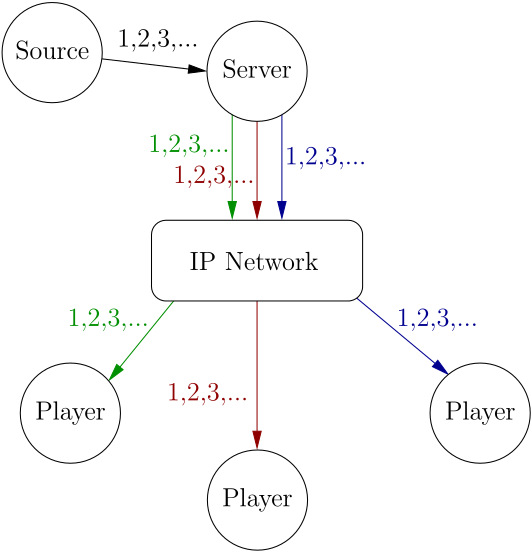
\includegraphics[width=1.0\textwidth]{unicast-server}
%\end{center}
\else
\HCode{
  <div style="text-align:center;">
    <img height="600" src="FIGs/unicast-server.svg" />
  </div>
}
\fi
% <object
%   height="750" data="unicast-hub.svg" type="image/svg+xml" align="middle" 
% </object>
% }

\section{IP-TV over IP Multicast}
\ifx \HCode\Undfef
%\begin{center}
%  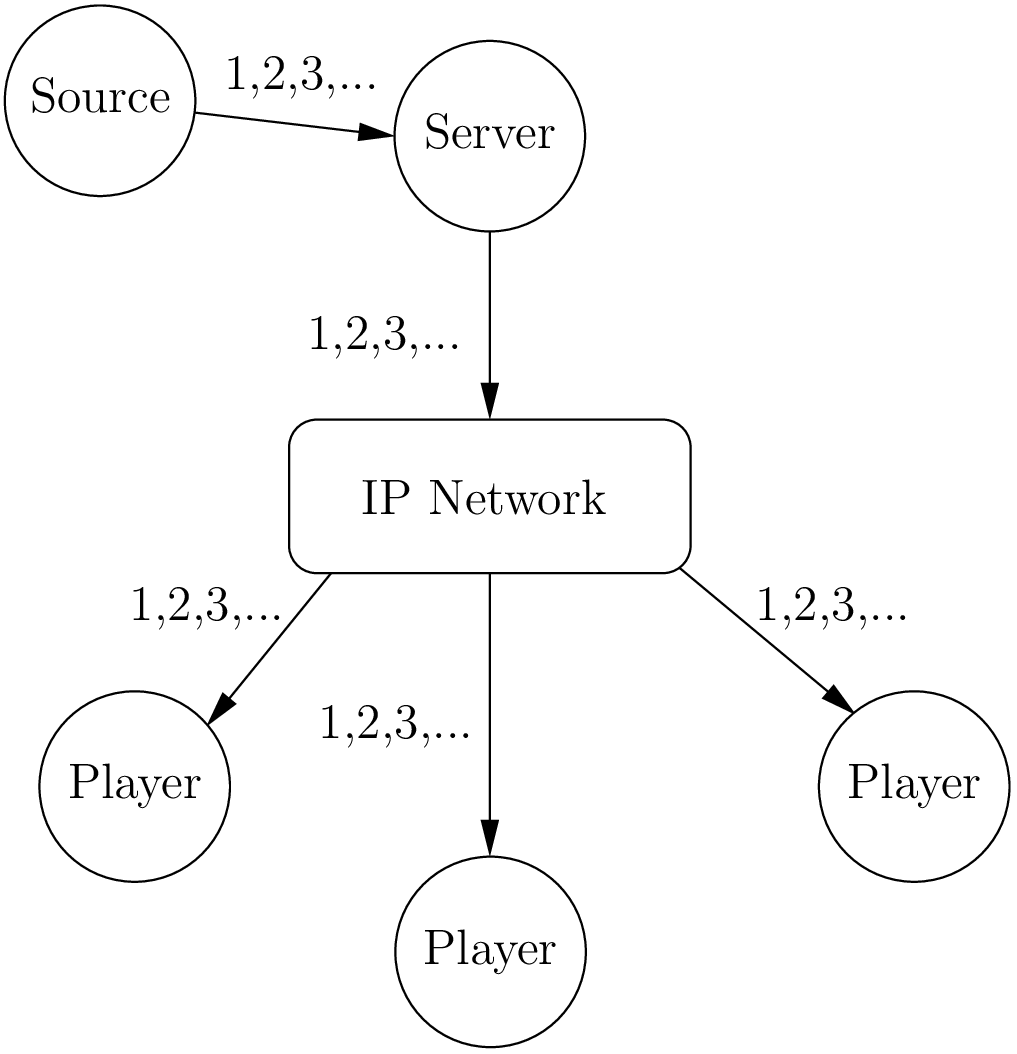
\includegraphics[width=1.0\textwidth]{multicast-server}
%\end{center}
\else
\HCode{
  <div style="text-align:center;">
    <img height="600" src="FIGs/multicast-server.svg" />
  </div>
}
\fi

\section{IP-TV over IP Unicast + P2PSP}
\ifx \HCode\Undfef
%\begin{center}
%  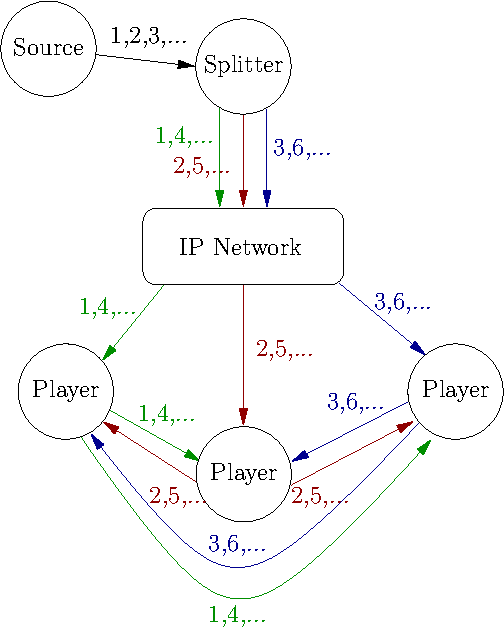
\includegraphics[width=1.0\textwidth]{unicast-splitter}
%\end{center}
\else
\HCode{
  <div style="text-align:center;">
    <img height="600" src="FIGs/unicast-splitter.svg" />
  </div>
}
\fi

\section{IP-TV over IP Unicast + P2PSP (revisited)}
\ifx \HCode\Undfef
%\begin{center}
%  \includegraphics[width=1.0\textwidth]{spain-IPTV-P2P}
%\end{center}
\else
\HCode{
  <div style="text-align:center;">
    <img height="600" src="FIGs/spain-IPTV-P2P.svg" />
  </div>
}
\fi

\section{Some words about P2PSP}
\begin{itemize}

\item \href{http://www.p2psp.org/en/}{P2PSP (Peer-to-Peer ``Straightforward'' Protocol)} is an open
  (\href{http://www.oxforddictionaries.com/definition/english/non-proprietary}{non-propietary})
  application-layer protocol for the real-time streaming of media
  content between networked entities.
\item An open-source (\href{https://www.gnu.org/copyleft/gpl.html}{GNU
    GPL v3}) implementation is available at
  \href{https://launchpad.net/p2psp}{Lauchpad}.
\end{itemize}

% \section{P2PSP architecture vs. C/S architecture.}
% \begin{center}
%   \includegraphics[width=0.9\textwidth]{P2PSP_vs_CS}
% \end{center}
% Notice that:
% \begin{enumerate}
% \item The P2PSP's Splitter node (S in red) only sends a copy of the
%   stream regardless of the number of Peers (P). In a C/S system, the
%   Server (S in green) sends as many copies as Clients (C).
% \item If a link or a Peer fails in a P2PSP team, the lost chunks are
%   dispersed in time. Therefore, signal interpolation could be
%   efficiently used to hide to the users this lost of information.
% \end{enumerate}

\large
\section{P2PSP's Sets of Rules}
\begin{enumerate}
\item \textbf{IP Mulicast Set:} The splitter sends the chunks to
  the peers using a IP multicast channel. Peers do not communicate
  each other.

\ifx \HCode\Undfef
%\begin{center}
%  \includegraphics[width=0.5\textwidth]{multicast-splitter}
%\end{center}
\else
\HCode{
  <div style="text-align:center;">
    <img height="600" src="FIGs/multicast-splitter.svg" />
  </div>
}
\fi

\item \textbf{Data Broadcasting Set:} IP multicast is not available? Then, all nodes must contribute
  equally (send the same amount of data) using unicast transmissions.

\ifx \HCode\Undfef
%\begin{center}
%  \includegraphics[width=0.5\textwidth]{congestion_control}
%\end{center}
\else
\HCode{
  <div style="text-align:center;">
    <img height="800" src="FIGs/congestion_control.svg" />
  </div>
}
\fi

\item \textbf{Adaptive Chunk-rate Set:} Peers can send a different
  amount of data, depending on their estimated bandwidth.

\ifx \HCode\Undfef
%\begin{center}
%  \includegraphics[width=0.5\textwidth]{ACS}
%\end{center}
\else
\HCode{
  <div style="text-align:center;">
    <img height="300" src="FIGs/ACS.svg" />
  </div>
}
\fi

\item \textbf{Lost chunks Recovery Set:} Retransmit massively lost
  chunks.

\ifx \HCode\Undfef
%\begin{center}
%  \includegraphics[width=0.5\textwidth]{FIGs/LRS}
%\end{center}
\else
\HCode{
  <div style="text-align:center;">
    <img height="500" src="FIGs/LRS.svg" />
  </div>
}
\fi

\item \textbf{End-point Masquerading Set:} Allows that two or more peers can
  run behind the same full-cone NAT (in the same private network).

\ifx \HCode\Undfef
%\begin{center}
%  \includegraphics[width=0.5\textwidth]{FIGs/EMS}
%\end{center}
\else
\HCode{
  <div style="text-align:center;">
    <img width="800" src="FIGs/EMS.svg" />
  </div>
}
\fi

\item \textbf{NAT Traversal Set:} Extra functionality to (\emph{try
    to}) handle peers that are behind restricted-cone NATs and
  symmetric NATs.

\item \textbf{Multi-Channel Set:} Communicates with several teams
  (channels) concurrently. This can be usefull, for example, to
  streming 3D video.

\ifx \HCode\Undfef
%\begin{center}
%  \includegraphics[width=0.5\textwidth]{3d-example}
%\end{center}
\else
\HCode{
  <div style="text-align:center;">
    <img height="500" src="FIGs/3d-example.svg" />
  </div>
}
\fi

\item \textbf{Content Integrity Set:} Rules against the poisoning
  of the stream, DoS (Denial of Service) attacks, etc.

\item \textbf{Data Privacy Set:} To implement, for
  example, pay-per-view services.

\end{enumerate}
\normalsize

\part*{Demos}
\begin{enumerate}
\item \href{https://www.youtube.com/watch?v=R7035-XaZd4}{Testing an implementation of the P2PSP using WebRTC.}

\ifx \HCode\Undfef
\else
\HCode{
<iframe width="560" height="315" src="http://www.youtube.com/embed/R7035-XaZd4?t=1m3s" frameborder="0" allowfullscreen></iframe>
</iframe> 
}
\fi

% \ifx \HCode\Undfef
% \else
% \HCode{
% <?php header('X-Frame-Options: GOFORIT'); ?>
% <iframe width="560" height="315" src="https://www.youtube.com/watch?v=R7035-XaZd4" frameborder="0" allowfullscreen></iframe>
% <iframe width="560" height="315" src="//www.youtube.com/embed/R7035-XaZd4" frameborder="0" allowfullscreen></iframe>
% }
% \fi

\item \href{https://www.youtube.com/watch?v=sB3u9U49woM}{Testing ``The P2PSP Test Pattern Channel''.}

\ifx \HCode\Undfef
\else
\HCode{
<iframe width="560" height="315" src="http://www.youtube.com/embed/sB3u9U49woM?t=1m3s" frameborder="0" allowfullscreen></iframe>
}
\fi

\end{enumerate}

\part*{}
\begin{center}
~\\
~\\
~\\
\Huge{Thanks!}
~\\
~\\
~\\
~\\
\end{center}

\end{document}
